% =========================================================================== %
% Yes. This is a document.

\documentclass[
	english,
	aspectratio=169,
	table
]{beamer}

% =========================================================================== %
% Theme
\usepackage{scrlfile}
	\ReplacePackage{beamerthemeSHUR}{./sty/beamerthemeSHUR}
	\ReplacePackage{beamerinnerthemefancy}{./sty/beamerinnerthemefancy}
	\ReplacePackage{beamerouterthemedecolines}{./sty/beamerouterthemedecolines}
	\ReplacePackage{beamercolorthemechameleon}{./sty/beamercolorthemechameleon}

\usetheme[
	pageofpages=/,
	bullet=circle,
	titleline=true,
	alternativetitlepage=true,
	watermark="",
	watermarkheight=0px,
	watermarkheightmult=0
	]
{SHUR}

% =========================================================================== %
% the usual stuff

\usepackage[utf8]{inputenc}
\usepackage[T1]{fontenc}
\usepackage{babel}
\usepackage{lmodern}
\usepackage{microtype}
\usepackage{csquotes}

\usepackage{tabularx}
\usepackage{booktabs}
\usepackage{multirow}

\usepackage{color, colortbl}
\usepackage{xcolor}
	\definecolor{tabhighlight}{RGB}{230,240,255}
	\definecolor{tabcontrast} {RGB}{200,210,255}

\usepackage{tabto}
\usepackage{xspace}

% math
\usepackage{amsmath}
\usepackage{amssymb}
\usepackage{dsfont}
\usepackage[arrowdel]{physics}
\usepackage{mathtools}
\usepackage{siunitx}

\usepackage{minted}
	\usemintedstyle{friendly}

\usepackage{tikz}
	\usetikzlibrary{positioning}
	\usetikzlibrary{matrix}
	\usetikzlibrary{shapes.geometric}
	\usetikzlibrary{backgrounds}
	\usetikzlibrary{calc}
	\usetikzlibrary{decorations.pathreplacing}
	\usetikzlibrary{arrows}
\usepackage{adjustbox}

\usepackage[most]{tcolorbox}
	\tcbsetforeverylayer
		{colback=cyan!10!white,
		 colframe=cyan!75!black,
		 arc=0pt,
		 outer arc=0pt,
		 parbox=false
		}
	\newtcolorbox{codebox}[1][Code]
		{colback=black!5!white,
		 colframe=blue!40!black,
		 title=#1,
		 leftupper=6mm
		}
	\newtcolorbox{cmdbox}[1][Kommandozeilen-Befehl]
		{colback=black,
		 coltext=white,
		 fontupper=\ttfamily ,
		 colframe=blue!40!black,
		 title=#1,
		 outer arc=0pt
		}
	\newtcolorbox{warnbox}[1][Beachte]
		{colback=black!5!white,
		 colframe=red!40!black,
		 title=#1
		}
	\newtcolorbox{hintbox}[1][Tipp]
		{colback=black!5!white,
		 colframe=green!40!black,
		 title=#1
		}
	\newenvironment{itembox}
		{\begin{tcolorbox}\begin{itemize}}%
		{\end{itemize}\end{tcolorbox}}
	\newtcolorbox{doublebox}[1][.3]
		{righthand width=#1\linewidth,
		 sidebyside,
		 sidebyside gap=6mm,
		 sidebyside align=center,
		 lower separated=false}
	
%==============================================================================%
% GLOBAL MACROS

\newcommand*{\eg}{e.\,g. }
\newcommand*{\ie}{i.\,e. }

\newcommand{\Thus}{\ensuremath{\Rightarrow}\xspace}
\newcommand{\thus}{\ensuremath{\rightarrow}\xspace}

\newcommand*{\tabcrlf}{\\ \midrule}			% actually still allows for optional argument

\newcommand*{\inPy}[1]{\mintinline{python3}{#1}}

% =========================================================================== %

\author{Stefan Hartinger}
\title{Programming in Python}
\subtitle{Part 15: Batch Processing with NumPy (II)}
\institute{University Regensburg, Department of Theoretical Physics}
\date{Winter Term 2021/22}

% =========================================================================== %

\begin{document}
% =========================================================================== %

\begin{frame}[t,plain]
\titlepage
\end{frame}

% =========================================================================== %

\begin{frame}{Recap}
%
\begin{columns}[T]
\column{.5\linewidth}
\begin{itemize}
\item \texttt{np.ndarray}
	\begin{itemize}
	\item Collection of objects of same type
	\item Arbitrary dimension, but fully defined
	\item Allows faster processing
	\end{itemize}
\item Indexing
	\begin{itemize}
	\item Like Python \inPy{list}s
	\item Or with \inPy{tuple}s and \inPy{slice}s
	\item Or with Bitmasks
	\end{itemize}
\item Quick Generation
	\begin{itemize}
	\item \texttt{np.linspace}, \texttt{np.arange}, \texttt{np.geomspace}, \texttt{np.logspace}
	\item \texttt{np.zeros}, \texttt{np.ones}, \texttt{np.fill}
	\item \texttt{np.identity}, \texttt{np.eye}, \texttt{np.diag}
	\end{itemize}
\end{itemize}
%
\column{.5\linewidth}
\begin{itemize}
\item Meshgrids
	\begin{itemize}
	\item Generates all conceivable combinations
	\item \inPy{list} of \texttt{np.ndarray}s
	\item Special form: \texttt{np.indices} for combinations of indices
	\end{itemize}
\item Broadcasting
	\begin{itemize}
	\item Element-Wise evaluation of operations
	\item With other \texttt{np.array}s of same dimension or with scalars
	\item Special Functions
	\item Comparison Operators
	\end{itemize}
\item Transpositions
	\begin{itemize}
	\item With attribute \texttt{T} or method \texttt{transpose}
	\end{itemize}
\end{itemize}

\end{columns}
%
\begin{center}
	\emph{Any Questions?}
\end{center}
%
\end{frame}

% =========================================================================== %

\begin{frame}[fragile]{Chapter 11}
%
\begin{itemize}
\item Reduction
\item Changing the Shape of an \texttt{np.ndarray}
\item Linear Algebra
\item Random Numbers
\end{itemize}
%
\end{frame}

% =========================================================================== %

\begin{frame}[fragile]{Reductions}
%
\begin{itemize}
\item Computing a single value from a collection of values
	\begin{itemize}
	\item E.\;g. sum, average, minimum, ...
	\end{itemize}
\item Involve at least one loop
\item Potential for exploitation of regular structure of \texttt{np.ndarray}s.
\item[\Thus] Numpy-Functions
	\begin{itemize}
	\item \texttt{np.sum}, \texttt{np.prod}
	\item \texttt{np.mean}, \texttt{np.median}, \texttt{np.average}
	\item \texttt{np.min}, \texttt{np.max}
	\item \texttt{np.argmin}, \texttt{np.argmax}
	\item \texttt{np.all}, \texttt{np.any}
	\end{itemize}

\end{itemize}
%
\end{frame}

% =========================================================================== %

\begin{frame}[fragile]{Measuring the Speedup}
%
\begin{itemize}
\item Module \texttt{time}: Functions for dealing with measuring and displaying passage of time
\item Internally: time as a floating point value
	\begin{itemize}
	\item Number of seconds since a given \emph{epoch}
	\item Usually: Linux epoch, 1970-01-01, 00:00
	\item Alternative (high precision time \emph{differences}): Seconds since start of system
	\end{itemize}
\item Function \texttt{time.time()} -- seconds since Linux epoch
\item Function \texttt{time.perf\_counter()} -- seconds since booting the computer
\item Time difference very small, subject to fluctuations
\item Measure repeatedly, compute average
\end{itemize}
%
\end{frame}

% =========================================================================== %

\begin{frame}[fragile]
%
\vspace{-3pt}
\begin{codebox}[Example: Speedup in Summation due to NumPy]
\begin{minted}[linenos, fontsize=\scriptsize]{python3}
import numpy as np; import time
N = 10000; R = 2000; X = np.linspace(0, 100, N)

print(f"taking time for summation of {N} values, Python-Style...", end="", flush=True)
tic = time.perf_counter()
for run in range(R) : s = sum(X)
toc = time.perf_counter()
tPython = toc - tic
print("done")

print(f"taking time for summation of {N} values, NumPy-Style...", end="", flush=True)
tic = time.perf_counter()
for run in range(R) : s = np.sum(X)
toc = time.perf_counter()
tNumpy = toc - tic
print("done", end="\n\n")

print(f"Measured {tPython*1000/R:5.3f} milliseconds using the Python-Method")
print(f"Measured {tNumpy *1000/R:5.3f} milliseconds using the NumPy-Method")
print(f"NumPy is {tPython/tNumpy:5.1f} times faster than native Python")
\end{minted}
\end{codebox}
%
\end{frame}

% =========================================================================== %

\begin{frame}[fragile]
%
\vspace{-3pt}
\begin{cmdbox}[Output: Speedup in Summation due to NumPy]
\begin{minted}[fontsize=\scriptsize]{text}
taking the time for summation of 10000 values, Python-Style...done
taking the time for summation of 10000 values, NumPy-Style...done

Measured 0.850 milliseconds using the Python-Method
Measured 0.007 milliseconds using the NumPy-Method
NumPy is 120.8 times faster than native Python
\end{minted}
\end{cmdbox}
%
\begin{itemize}
\item Part of this success due to: NumPy is \emph{compiled to machine language} rather than to \emph{bytecode}
\item \enquote{Request is formulated in the computer's language, without prior need to translate}
\item Depending on the task, a factor 10 ... 1000 can be gained by choosing a compiled language over an interpreted one
\end{itemize}
%
\end{frame}

% =========================================================================== %

\begin{frame}[fragile]{Difference between \texttt{np.mean} and \texttt{np.average}}
%
\begin{itemize}
\item Both can do the same, but \texttt{np.average} can do more
\item \texttt{np.mean(A)} computes $\frac{1}{N} \sum_{i=1}^{N} A_i$
\item \texttt{np.average(A, weights=w)} computes weighted average (and optionally partition function)
	\begin{itemize}
	\item Partition function $Z = \sum_{i=1}^{N} w_i$
	\item Weighted average $\text{wa}(A, w) = \frac{1}{Z} \sum_{i=1}^{N} A_i w_i$
	\item To get only the weighted average, use signature \texttt{np.average(A, weights=w)}
	\item To get a tuple of weighted average and partition funciton, sude signature \texttt{np.average(A, weights=w, returned=True)}
	\end{itemize}
\end{itemize}
%
\end{frame}

% =========================================================================== %

\begin{frame}[fragile]
%
\begin{codebox}[Example: Average Speed of Hydrogen Atoms]
\begin{minted}[linenos, fontsize=\scriptsize]{python3}
kB = 1.380649e-23         # Boltzmann constant
T  = 300                  # Temperature in Kelvin
m  = 2 * 1.6735575e-27    # hydrogen molecule mass in kg

velocities = np.linspace(0, 5000, 50000)
energies   = m/2 * velocities**2
w = np.exp(-energies / (kB * T))

vMean, Z = np.average(velocities * 2, weights=w, returned=True)

print("weighted average                     :", vMean, "m/s")
print("mean of the magnitude of the velocity:", np.sqrt((8*kB*T)/(m*np.pi)), "m/s" )
print("partition function                   :", Z, "J")
\end{minted}
\end{codebox}
%
\end{frame}

% =========================================================================== %

\begin{frame}
%
\begin{tcolorbox}[title=For Physicists]
\vspace{6pt}
Expectation value:
\tabto{5cm}
$ \displaystyle \expval{A} = \frac{1}{Z} \int_0^{\infty} \dd{E} \; A(E) \exp(\frac{-E}{k_B T}) $

\vspace{9pt}
Change of integration variable:
\tabto{5cm}
$ \displaystyle \expval{A} = \frac{1}{Z} \int_A \dd{A} \dv{E}{A} \; A \exp(\frac{-E(A)}{k_B T}) $

\vspace{15pt}
In the case of velocity:
\tabto{5cm}
$ \displaystyle E(v) = \frac{m}{2} v^{2} $\\
\vspace{9pt}
\tabto{5cm}
$ \displaystyle \dv{E}{v} = mv $

\vspace{9pt}
Together:
\tabto{5cm}
$ \displaystyle 
	\expval{v}
=
	\frac{1}{Z}
	\int_0^{\infty} \dd{v} 
		\underbrace{		
			mv \cdot v
		}_{2E(v)}
		\cdot \exp(\frac{-\frac{m}{2} v^2}{k_B T}) $

\vspace{9pt}
\Thus Factor 2 in line 9 on the last slide
\end{tcolorbox}
%
\end{frame}

% =========================================================================== %

\begin{frame}[fragile]{Reduction of Multidimensional Arrays -- \texttt{axis}-Mechanism}
%
\begin{itemize}
\item What should \texttt{np.sum(matrix)} be?
	\begin{itemize}
	\item Sum of all numbers?
	\item Vector of row-sums?
	\item Vector of column-sums?
	\end{itemize}
\item NumPy can do all of them!
\item Needed information: sum along which direction \Thus \texttt{axis}
	\begin{itemize}
	\item \inPy{int}, specifying the \emph{number of the index} along which summation takes place
	\item Default: \inPy{None}, which means \emph{sum all values}
	\item Example: \inPy{np.sum(matrix, axis=0)}: equivalent to \inPy{matrix[0, :] + matrix[1, :] + ...}
	\item Example: \inPy{np.sum(matrix, axis=1)}: equivalent to \inPy{matrix[:, 0] + matrix[:, 1] + ...}
	\item[\Thus] \texttt{axis} specifies which dimension to reduce
	\end{itemize}
\item Same concept for other reduction functions and higher dimensional objects (tensors)
\end{itemize}
%
\end{frame}

% =========================================================================== %

\begin{frame}[fragile]{Changing the Shape of \texttt{np.ndarray}s (I)}
%
\begin{itemize}
\item Method \texttt{array.resize(new\_size)}
	\begin{itemize}
	\item \texttt{new\_size}: \inPy{tuple} with new dimensions
	\item If bigger: fill with zeros
	\item If smaller: \enquote{forget} values
	\end{itemize}
\item Somewhat unintuitive:
	\begin{itemize}
	\item Let $\displaystyle A = \mqty(1 & 2 \\ 3 & 4)$ and do \texttt{A.resize((2, 3))}
	\item Get $\displaystyle A = \mqty(1 & 2 & 3 \\ 4 & 0 & 0)$
	\end{itemize}
\item Reason: Vectorization
	\begin{itemize}
	\item Internally, \texttt{A} is just a string of numbers plus \inPy{tuple} for shape
	\item \texttt{A "=" [(2, 2), 1, 2, 3, 4]}
	\item Method \texttt{resize} only appends zeros to the data and updates \texttt{shape}
	\item[\Thus] \texttt{A "=" [(2, 3), 1, 2, 3, 4, 0, 0]}
	\end{itemize}
\end{itemize}
%
\end{frame}

% =========================================================================== %

\begin{frame}[fragile]{Chnging the Shape of \texttt{np.ndarray}s (II)}
%
\begin{itemize}
\item Related method: \texttt{reshape}
	\begin{itemize}
	\item Changes \inPy{tuple shape}
	\item Does not affect the stored data itself
	\item Raises an error if change would add/remove data
	\end{itemize}
\item Example:
	\begin{itemize}
	\item Let $\displaystyle A = \mqty(1 & 2 & 3 & 4)$ and do \texttt{A.reshape((2, 2))}
	\item Get $\displaystyle A = \mqty(1 & 2 \\ 3 & 4)$
	\item Do \texttt{A.reshape((5,))}
	\item Get \texttt{ValueError: cannot reshape array of size 4 into shape (5,)}
	\end{itemize}
\item Permanence
	\begin{itemize}
	\item \texttt{resize} changes an array permanently
	\item \texttt{reshape} creates \enquote{a new view} on the same data
	\end{itemize}
\end{itemize}
%
\end{frame}

% =========================================================================== %

\begin{frame}[fragile]
%
\vspace{-3pt}
\begin{tcolorbox}[title=Memory Model: \texttt{np.ndarray}s]
\begin{codebox}[Example: Different Views]
\begin{minted}[fontsize=\scriptsize, linenos]{python3}
data = np.array([[1, 2], [3, 4]])
view = data.reshape((4,))
\end{minted}
\end{codebox}
%
\begin{center}
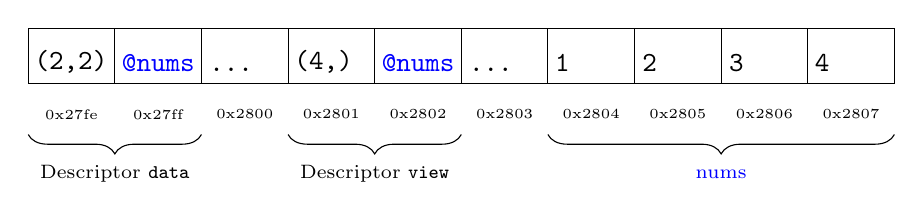
\begin{tikzpicture}
  [ 
    cell/.style={
      text width=9mm,
      text height=4mm,
      draw=black,
      inner sep=1mm,
      minimum height=7mm
    },
    ld/.style={draw=blue,shorten >=2pt,->}
  ]
  \node (a0) at (0.0,4) [cell] {\ttfamily (2,2)};
  \node (a1) at (1.1,4) [cell] {\ttfamily {\color{blue} @nums}};
  \node (a2) at (2.2,4) [cell] {\ttfamily ...};
  \node (a3) at (3.3,4) [cell] {\ttfamily (4,)};
  \node (a4) at (4.4,4) [cell] {\ttfamily {\color{blue} @nums}};
  \node (a5) at (5.5,4) [cell] {\ttfamily ...};
  \node (a6) at (6.6,4) [cell] {\ttfamily 1};
  \node (a7) at (7.7,4) [cell] {\ttfamily 2};
  \node (a8) at (8.8,4) [cell] {\ttfamily 3};
  \node (a9) at (9.9,4) [cell] {\ttfamily 4};
  
  \node (A0) [below=2mm of a0] {\tiny 0x27fe};
  \node (A1) [below=2mm of a1] {\tiny 0x27ff};
  \node (A2) [below=2mm of a2] {\tiny 0x2800};
  \node (A3) [below=2mm of a3] {\tiny 0x2801};
  \node (A4) [below=2mm of a4] {\tiny 0x2802};
  \node (A5) [below=2mm of a5] {\tiny 0x2803};
  \node (A6) [below=2mm of a6] {\tiny 0x2804};
  \node (A7) [below=2mm of a7] {\tiny 0x2805};
  \node (A8) [below=2mm of a8] {\tiny 0x2806};
  \node (A9) [below=2mm of a9] {\tiny 0x2807};


  \draw [decorate, decoration={brace,amplitude=7pt, mirror}, xshift=-0pt, yshift=0pt]
  		(-0.55, 3.0) -- (1.65, 3.0) node [midway, yshift=-0.5cm] 
		(bracedata) {\scriptsize Descriptor \texttt{data}};
  \draw [decorate, decoration={brace,amplitude=7pt, mirror}, xshift=-0pt, yshift=0pt]
  		( 2.75, 3.0) -- (4.95, 3.0) node [midway, yshift=-0.5cm] 
		(bracedata) {\scriptsize Descriptor \texttt{view}};
  \draw [decorate, decoration={brace,amplitude=7pt, mirror}, xshift=-0pt, yshift=0pt]
  		( 6.05, 3.0) -- (10.45, 3.0) node [blue, midway, yshift=-0.5cm] 
		(braceNums) {\scriptsize nums};

  \end{tikzpicture}
\end{center}
%
\begin{tcbraster}[raster columns=2,
                  raster equal height,
                  nobeforeafter,
                  raster column skip=0.5cm]
\begin{codebox}[Example: view changes data]
\begin{minted}[fontsize=\scriptsize, linenos, firstnumber=last]{python3}
view[3] = 0
print(data)
\end{minted}
\end{codebox}
%
\begin{cmdbox}[Output: view changes data]
\begin{minted}[fontsize=\scriptsize]{text}
[[1, 2]
 [3, 0]]
\end{minted}
\end{cmdbox}
\end{tcbraster}
\end{tcolorbox}
%
\end{frame}

% =========================================================================== %

\begin{frame}[fragile]
%
\begin{hintbox}[Copying \texttt{np.ndarray}s]
Like Python \inPy{list}s, you can use the module \texttt{copy} to get a copy rather than a reference. Much better still is to use the method \texttt{copy} of \texttt{np.ndarray}s, which exploits the regular structure and hence works much faster than Python's native copy.
\end{hintbox}
%
\begin{warnbox}[Slices create views{,} too]
Unlike Python, using slices does \emph{not} copy the content of \texttt{np.ndarray}s:

\vspace{4pt}
\begin{tcbraster}[raster columns=2,
                  raster equal height,
                  nobeforeafter,
                  raster column skip=0.5cm]
\begin{codebox}[Example: View from Slices]
\begin{minted}[fontsize=\scriptsize, linenos]{python3}
data = np.array([[1,2,3],[4,5,6]])
view = data[:, 1:]
view[1,1] = 0
print(data)
\end{minted}
\end{codebox}
%
\begin{cmdbox}[Output: View from Slices]
\begin{minted}[fontsize=\scriptsize]{text}
[[1, 2, 3]
 [4, 5, 0]]
\end{minted}
\end{cmdbox}
\end{tcbraster}

\end{warnbox}
%
\end{frame}

% =========================================================================== %

\begin{frame}[fragile]{Concatenation, Insertion, Deletion}
%
\begin{itemize}
\item Joining two arrays
	\begin{itemize}
	\item \texttt{np.concatenate(what, axis=0)}
	\item \texttt{what} is a \inPy{tuple} mentioning all \texttt{np.ndarray}s to concatenate
	\item All elements in \texttt{what} need to be of same dimension
	\item \texttt{axis} can be none (creates a 1D list of all elements)
	\end{itemize}
\item Inserting data
	\begin{itemize}
	\item \inPy{np.insert(array, where, what, axis=0)}
	\item \texttt{array} specifies, into which array insertion should be made
	\item \texttt{where} is a \inPy{tuple} specifying where to insert data
	\item \texttt{what} is the data to be inserted. Can be a scalar (will be repeated) or an array
	\end{itemize}
\item Both functions return a copy with the inserted data
\item Numpy Reference
	\begin{itemize}
	\item \scriptsize \url{https://numpy.org/doc/stable/reference/generated/numpy.concatenate.html}
	\item \scriptsize \url{https://numpy.org/doc/stable/reference/generated/numpy.insert.html}
	\end{itemize}
\end{itemize}
%
\end{frame}

% =========================================================================== %

\begin{frame}[fragile]
%
\begin{tcbraster}[raster columns=2,
                  raster equal height,
                  nobeforeafter,
                  raster column skip=0.2cm]
\begin{codebox}[Example: \texttt{np.concatenate}]
\begin{minted}[fontsize=\scriptsize, linenos]{python3}
import numpy as np

a = np.array([[1, 2], [3, 4]])
b = np.array([[5, 6]])

print(np.concatenate((a, b)))
print()
print(np.concatenate((a, b), axis=0))
print()
print(np.concatenate((a, b.T), axis=1))
print()
print(np.concatenate((a, b), axis=None))
\end{minted}
\end{codebox}
%
\begin{cmdbox}[Output: \texttt{np.concatenate}]
\begin{minted}[fontsize=\scriptsize]{text}
[[1 2]
 [3 4]
 [5 6]]
 
[[1 2]
 [3 4]
 [5 6]]

[[1 2 5]
 [3 4 6]]

[1 2 3 4 5 6]
\end{minted}
\end{cmdbox}
\end{tcbraster}
%
\end{frame}

% =========================================================================== %

\begin{frame}[fragile]
%
\begin{tcbraster}[raster columns=2,
                  raster equal height,
                  nobeforeafter,
                  raster column skip=0.2cm]
\begin{codebox}[Example: \texttt{np.concatenate}]
\begin{minted}[fontsize=\scriptsize, linenos]{python3}
data = np.array([0, 1, 2, 3],
                [4, 5, 6, 7])
idx = (1, 3)
print( np.insert(data, 
                 idx, 999, axis=1) )
print()

data = np.array([[1, 1],
                 [2, 2],
                 [3, 3]])
print( np.insert(data, 1, 5) )
print()

print( np.insert(data, 1, 5, axis=1) )
print()

print( np.insert(data,
                [1], [[1],[2],[3]],
                axis=1) )
\end{minted}
\end{codebox}
%
\begin{cmdbox}[Output: \texttt{np.concatenate}]
\begin{minted}[fontsize=\scriptsize]{text}
[[  0 999   1   2 999   3]
 [  4 999   5   6 999   7]]
 
[1 5 1 2 2 3 3]

[[1 5 1]
 [2 5 2]
 [3 5 3]]
 
[[1 1 1]
 [2 2 2]
 [3 3 3]]
\end{minted}
\end{cmdbox}
\end{tcbraster}
%
\end{frame}

% =========================================================================== %

\begin{frame}[fragile]{More Functions}
%
\begin{itemize}
\item Split arrays: \texttt{np.split}
	\begin{itemize}
	\item \scriptsize \url{https://numpy.org/doc/stable/reference/generated/numpy.split.html}
	\end{itemize}
\item Delete sub-arrays: \texttt{np.delete}
	\begin{itemize}
	\item \scriptsize \url{https://numpy.org/doc/stable/reference/generated/numpy.delete.html}
	\end{itemize}
\item Join Arrays of different dimension: \texttt{np.stack}
	\begin{itemize}
	\item \scriptsize \url{https://numpy.org/doc/stable/reference/generated/numpy.stack.html}
	\end{itemize}
\item Making arrays 1D: \texttt{np.flatten}
	\begin{itemize}
	\item \scriptsize \url{https://numpy.org/doc/stable/reference/generated/numpy.flatten.html}
	\end{itemize}
\item Repat contents of arrays: \texttt{np.repeat} and \texttt{np.tile}
	\begin{itemize}
	\item \scriptsize \url{https://numpy.org/doc/stable/reference/generated/numpy.repeat.html}
	\item \scriptsize \url{https://numpy.org/doc/stable/reference/generated/numpy.tile.html}
	\end{itemize}
\item Rearrange arrays: \texttt{np.roll}
	\begin{itemize}
	\item \scriptsize \url{https://numpy.org/doc/stable/reference/generated/numpy.roll.html}
	\end{itemize}
\item Sort arrays: \texttt{np.sort}
	\begin{itemize}
	\item \scriptsize \url{https://numpy.org/doc/stable/reference/generated/numpy.sort.html}
	\end{itemize}
\item ...
\end{itemize}
%
\end{frame}

% =========================================================================== %

\begin{frame}{Linear Algebra}
%
\vspace{-6pt}
\begin{tcolorbox}[title=Wikipedia]
\scriptsize
Linear algebra is the branch of mathematics concerning linear equations such as:
\[ a_{1} x_{1} + \cdots + a_{n} x_{n} = b \]
\end{tcolorbox}
%
\begin{itemize}
\item Linear Algebra is often formulated in terms of matrices
\item Many Real World Applications
\item NumPy has an own submodule dedicated to solving problems from linear algebra
\item Linear: all variables at most to the first power
\item Examples for \emph{nonlinear} terms
	\vspace{-6pt}
	\begin{columns}
	\column{.45\linewidth}
	\vspace{-6pt}
	\begin{itemize}
	\item $x^2 = 2$
	\item $x \cdot y = 5$
	\end{itemize}
	%
	\column{.45\linewidth}
	\begin{itemize}
	\item $\sin(x)$
	\item $f(x) = \begin{cases}
		0 & \text{if } x < 0 \\
		1 & \text{if } x \geq 0
	\end{cases}$
	\end{itemize}
	\end{columns}
\end{itemize}
%
\end{frame}

% =========================================================================== %\\

\begin{frame}[fragile]{Systems of Linear Equations}
%
\begin{itemize}
\item Several linear equations that need to be satisfied at the same time
\item As many variables as equations
\item Implicit question: which values for the variables solve the system of equations?
\item Step 1: Transform in to \emph{coefficient matrix} and \emph{inhomogeneity vector}
\item Step 2: Pass to \texttt{np.linalg.solve}
\item Step 3: Profit
\end{itemize}
%
\begin{tcbraster}[raster columns=2,
                  raster equal height,
                  nobeforeafter,
                  raster column skip=0.2cm]
\begin{tcolorbox}[title=Example]
\begin{align*}
	 x + 2y - 5z &=  7 \\
	8x - 3y + 2z &=  1 \\
	     9y - 9z &= -2
\end{align*}
\end{tcolorbox}
%
\begin{tcolorbox}[title=Coefficient Matrix{,} Inhomogeneity]
\begin{align*}
\scriptsize
A = \begin{pmatrix}
	1 &  2 & -5 \\
	8 & -3 &  2 \\
	0 &  9 & -9
\end{pmatrix}
~
b = \mqty(7 \\ 1 \\ -2)
~
v = \mqty(x \\ y \\ z)
\end{align*}

System as matrix equation: $Av = b$
\end{tcolorbox}
\end{tcbraster}
%
\end{frame}

% =========================================================================== %

\begin{frame}[fragile]
%
\begin{codebox}[Example: \texttt{linalg.solve}]
\begin{minted}[linenos, fontsize=\scriptsize]{python3}
coeffs = np.array( [[1,  2, -5],
                    [8, -3,  2],
                    [0,  9, -9]] )
inhom = np.array([7, 1, -2])

print( np.linalg.solve(coeffs, inhom) )
\end{minted}
\end{codebox}
%
\begin{cmdbox}[Output: \texttt{linalg.solve}]
\begin{minted}[fontsize=\scriptsize]{text}
[-0.28019324 -2.79710145 -2.57487923]
\end{minted}
\end{cmdbox}
%
\end{frame}

% =========================================================================== %\\

\begin{frame}[fragile]{Unsolveable Systems of Linear Equations}
%
\begin{itemize}
\item Some systems have no solution at all
	\vspace{-12pt}
	\begin{align*}
		x + 2y = 2 \\
		2x + 4y = 5
	\end{align*}
\item Some systems have an infinite number of solutions
	\vspace{-12pt}
	\begin{align*}
		x + 2y = 2 \\
		2x + 4y = 4
	\end{align*}
	\vspace{-12pt}
	(All solutions satisfy $y = 1 - \frac{x}{2}$
	\vspace{14pt})
\item Common property: one line of the coefficient matrix is a multiple of the other
\item Generalization: \emph{Determinant} is zero
	\begin{itemize}
	\item Complex mathematical operation
	\item assigns each square matrix a single number
	\end{itemize}
\item \texttt{np.linalg.det}
\end{itemize}
%
\end{frame}

% =========================================================================== %

\begin{frame}[fragile]
%
\begin{codebox}[Example: \texttt{linalg.det}]
\begin{minted}[linenos, fontsize=\scriptsize]{python3}
coeffs = np.array( [[1, 2],
                    [2, 4]] )

print( np.linalg.det(coeffs) )  # output: 0
\end{minted}
\end{codebox}
%
\begin{warnbox}[Comparing to Zero]
\footnotesize
Never write something like

\mint{python3}{if np.linalg.det(A) == 0 :}

In the process of computing the determinant, small errors accumulate. In the end, you often get a result \emph{close to 0}, but not equal to zero. For that reason, rather check whether the modulus of the determinant is less than some small threshold:

\mint{python3}{if np.abs(np.linalg.det(A)) < epsilon :}

Depending on your code, good values for \texttt{epsilon} are between \inPy{1e-7} and \inPy{1e-15}.
\end{warnbox}
%
\end{frame}

% =========================================================================== %

\begin{frame}[fragile]{Eigensystems}
%
\begin{itemize}
\item Effect of matrix multiplication $Ax$ on vector $x$: rotation and stretching
\item Some vectors: only stretched, not rotated
\item[\Thus] \emph{Eigenvectors} with \enquote{stretching factor} alias \emph{Eigenvalue}
\item (In general): $N \times N$ matrix \Thus $N$ different Eigenvalues and corresponding Eigenvectors
\item Used in all branches of science that apply maths
\item \texttt{np.linalg.eig} finds both, Eigenvalues and Eigenvectors
\item Returns a \inPy{tuple} \texttt{(eigenvalues, eigenvectors)}
	\begin{itemize}
	\item \texttt{eigenvalues} is an \texttt{np.ndarray} of all Eigenvalues
	\item \texttt{eigenvectors} is a 2D \texttt{np.ndarray} of all Eigenvectors
	\item Get the $i^{\text{th}}$ Eigenvector from \texttt{eigenvectors[:, i]}
	\end{itemize}
\item Note: Eigenvectors are \emph{not} normalized
\end{itemize}
%
\end{frame}

% =========================================================================== %

\begin{frame}{Example: Ants}
%
\begin{itemize}
\item Imagine: Species of ants
\item Individuals in three colours (red, green, blue)
\item Probability of colour of children depends on colour of mother
	\begin{itemize}
	\item E.\;g. red mother will have 30\% green children
	\end{itemize}
\item All nine probabilities known \Thus can be arranged in matrix $A$
\item Current population known \Thus can be arranged as vector $v$
\item[\Thus] Matrix product $Av$ gives composition of next generation
\item[\Thus] Eigenvectors are equilibrium states
\end{itemize}
%
\end{frame}

% =========================================================================== %

\begin{frame}[fragile]
%
\begin{tcbraster}[raster columns=2,
                  raster equal height,
                  nobeforeafter,
                  raster column skip=0.2cm]
\begin{codebox}[Example: Ants]
\begin{minted}[linenos, fontsize=\scriptsize]{python3}
import numpy as np

reprod = np.array([[0.7, 0.0, 0.0],
                   [0.3, 0.7, 1.0],
                   [0.0, 0.3, 0.0]])

eVals, eVecs = np.linalg.eig(reprod)

print("Eigenvalues:\n", eVals)
print("Eigenvectors:\n", eVecs)

pop = -eVecs[:, 1]

print("Composition of 1st gen:\n",
      pop)
print("Composition of 2nd gen:\n",
      reprod @ pop)
\end{minted}
\end{codebox}
%
\begin{cmdbox}[Output: Ants]
\begin{minted}[fontsize=\scriptsize]{text}
Eigenvalues:
 [-0.3  1.   0.7]
Eigenvectors:
 [[ 0.          0.          0.79555728]
 [ 0.70710678 -0.95782629 -0.5568901 ]
 [-0.70710678 -0.28734789 -0.23866719]]
Composition of 1st gen:
 [-0.          0.95782629  0.28734789]
Composition of 2nd gen:
 [0.         0.95782629 0.28734789]
\end{minted}
\end{cmdbox}
\end{tcbraster}
%
\end{frame}

% =========================================================================== %

\begin{frame}{Random Numbers}
%
\begin{itemize}
\item Dedicated Submodule \texttt{np.random}
\item Quick generation of \emph{arrays} of random numbers
	\begin{itemize}
	\item \texttt{size} parameter for most methods
	\item Can be an \inPy{int} \Thus 1D list
	\item or a \inPy{tuple} \Thus Tensor of random numbers
	\end{itemize}
\item Various distributions
	\begin{itemize}
	\item uniform
	\item normal
	\item laplace
	\item ...
	\end{itemize}
\item \texttt{np.random.<name of distribution>}
	\begin{itemize}
	\item different parameters, depending on distribution
	\item Example: \texttt{np.random.normal(mu, sigma, size)}
	\end{itemize}
\end{itemize}
%
\end{frame}

% =========================================================================== %

\begin{frame}{Explore the Reference}
%
\begin{itemize}
\item I could show you only the most important features in the limited time we have
\item I couldn't even show you all options to the commands I've presented
\item[\Thus] Take your time to explore the NumPy module yourself
	\begin{itemize}
	\item Tutorial\\
		\scriptsize \url{https://numpy.org/doc/stable/user/tutorials_index.html}
	\item Reference\\
		\scriptsize \url{https://numpy.org/doc/stable/reference/index.html}
	\end{itemize}
\end{itemize}
%
\end{frame}

% =========================================================================== %

\begin{frame}
%

\includegraphics[width=\linewidth]{./gfx/thatsall}
%
\end{frame}

\end{document}

% MAREI!!
% whom do I give credit? Where?